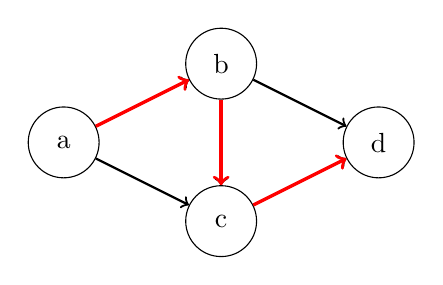
\begin{tikzpicture}[
    vertex/.style={circle, draw, minimum size=9mm, inner sep=0pt},
    edge/.style={->, thick},
    pathedge/.style={->, very thick, red}
]

    \node[vertex] (a) at (0,1.5) {a};
    \node[vertex] (b) at (2,2.5) {b};
    \node[vertex] (c) at (2,0.5) {c};
    \node[vertex] (d) at (4,1.5) {d};
    
    % Arestas do grafo
    \draw[edge] (a) -- (b);
    \draw[edge] (a) -- (c);
    \draw[edge] (b) -- (c);
    \draw[edge] (b) -- (d);
    \draw[edge] (c) -- (d);
    
    % Caminho destacado a -> b -> c -> d
    \draw[pathedge] (a) -- (b);
    \draw[pathedge] (b) -- (c);
    \draw[pathedge] (c) -- (d);

\end{tikzpicture}